\section{Experiments}
\label{sec:results}



\paragraph{Comparisons}
While our goal of enhancing given 3D assets with existing materials is distinct from recent work leveraging image models for view-consistent editing and generation, it is important to evaluate whether existing works can address our problem. \autoref{fig:baselines} justifies our technique by comparing it to related methods applied in our problem setting. The top half shows image generators that do not rely on the full 3D geometry of a given asset, including SPAD~\cite{spad}, Diffusion Handles~\cite{diffusion_handles}, and $\text{RGB}{\leftrightarrow}\text{X}$~\cite{RGBX}. Because SPAD and Diffusion Handles are not designed to work with the given 3D geometry of an input asset, they struggle to render the asset accurately from multiple viewpoints. On the other hand, $\text{RGB}{\leftrightarrow}\text{X}$ takes accurate scene intrinsics (normals, albedo, roughness, etc.) as input, but it is not equipped to ensure multi-view consistency.

The bottom part of \autoref{fig:baselines} compares our approach to DreamMat~\cite{dreammat} and TexPainter~\cite{TexPainter}, two state-of-the-art material generators for given 3D assets. While they focus on material generation from scratch, our primary goal is to enhance existing materials. Hence our result is more faithful to the initial asset provided as input (shown in \autoref{fig:hparams}), while also providing more realistic fine grained details. 



\begin{table}[h!]
    % \small
    \centering
    \caption{Links to baseline model checkpoints.}
    \resizebox{0.7\linewidth}{!}{
    \begin{tabular}{l|l}
    \toprule
    Model & URL \\
    \midrule
    Galactica 125M & \url{https://huggingface.co/facebook/galactica-125m}\\
    Galactica 1.3B& \url{https://huggingface.co/facebook/galactica-1.3b}\\
    Galactica 6.7B& \url{https://huggingface.co/facebook/galactica-6.7b}\\
    GIMLET & \url{https://huggingface.co/haitengzhao/gimlet}\\
    LlasMol & \url{https://huggingface.co/osunlp/LlaSMol-Mistral-7B}\\
    MolecularGPT & \url{https://huggingface.co/YuyanLiu/MolecularGPT}\\
    \bottomrule
    \end{tabular}}
    \label{app tab: baselines}
\end{table}

\paragraph{Visual results}
\autoref{fig:results} shows results of our complete pipeline, starting with basic assets, all the way to the recovered material parameters and the corresponding renderings.
The air conditioner result in particular highlights the advantage of using a diffusion model trained on natural images.
The rusting of the blades is distinct from that of the box itself, which aligns with the expectation these components would age differently.
In \autoref{fig:hparams_usercontrol} we show how classifier free guidance~\cite{ho2022cfg} enables the user to control the magnitude of the detail enhancements.
We show further examples in the supplementary document and video.

\begin{figure*}[htbp]
    \centering%
    \setlength{\tabcolsep}{0.002\textwidth}%
    \renewcommand{\arraystretch}{1}%
    \footnotesize%
    \begin{tabular}{ccccccc}
        Initial asset & \multicolumn{6}{c}{
            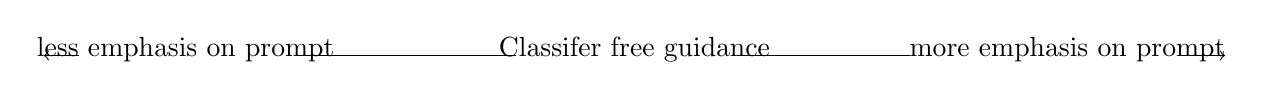
\begin{tikzpicture}
                \draw[<-] (0,0) -- (0.45,0);
                \draw[-] (3.2,0) -- (6.0,0);
                \draw[-] (8.8,0) -- (11,0);
                \draw[->] (14.4,0) -- (15,0);
                \node[above] at (1.8,-0.2) {less emphasis on prompt};
                \node[above] at (7.5,-0.2) {Classifer free guidance};
                \node[above] at (13,-0.2) {more emphasis on prompt};
            \end{tikzpicture}
        }\\[-4pt]%
        & 4.0 & \textbf{7.5} & 11.0 & 14.5 & 18.0 & 21.5\\%
        \includegraphics[height=0.14\linewidth]{figures/secondary_hparams/initial/0001.png}&%
        \includegraphics[height=0.14\linewidth]{figures/secondary_hparams/guidance_4.0_001.jpg}&%
        \includegraphics[height=0.14\linewidth]{figures/secondary_hparams/guidance_7.5_001.jpg}&%
        \includegraphics[height=0.14\linewidth]{figures/secondary_hparams/guidance_11.0_001.jpg}&%
        \includegraphics[height=0.14\linewidth]{figures/secondary_hparams/guidance_14.5_001.jpg}&%
        \includegraphics[height=0.14\linewidth]{figures/secondary_hparams/guidance_18.0_001.jpg}&%
        \includegraphics[height=0.14\linewidth]{figures/secondary_hparams/guidance_21.5_001.jpg}
    \end{tabular}%
    \caption{Controlling the magnitude of detail enhancements using classifier free guidance.
    The scaling factor allows the user to apply more conservative changes and stay closer to the input or obtain more pronounced changes, as desired.}
    \label{fig:hparams_usercontrol}
\end{figure*}


\paragraph{Ablation}
We validate our contributions and algorithmic choices to achieve view consistency of a pure 2D generative diffusion model by performing an ablation study presented in Figure~\ref{fig:ablation}.
We modify the appearance and detail of two 3D assets: a briefcase and a vase.
Pure ControlNet Tile is able to modify the appearance of the object with respect to the initial material, but fails to achieve view consistency.
Using view-correlated noise (Section.~\ref{sec:noise_warping}) we enhance the detail presence between different camera views, but some of the detail remains misaligned.
Finally, our full model that biases attention (Section.~\ref{sec:attention_bias}) further increases the consistency.

\paragraph{View consistency and inverse rendering}

Intuitively, view consistency between produced outputs is necessary to successfully reconstruct the material maps through inverse rendering.
When different views of the same surface \textit{disagree} and present different details, the inverse rendering process produces blurry results or fails to converge.
We present this effect in Figure~\ref{fig:invrender_inconsistent}.




